\documentclass[article]{beamer}% para se tiver muitas sections

\usetheme{Warsaw}
%====================================================================

\usefonttheme[]{serif}
\usepackage{amsmath, latexsym, color, graphicx, amssymb, bm, here}
\usepackage{epsf, epsfig, pifont,tikz,subfigure}
\usepackage{graphics, calrsfs}
\usepackage{times}
\usepackage{fancybox,calc}
\usepackage{palatino,mathpazo}
\usepackage{amsfonts}
\usepackage{wrapfig}
\usepackage{multicol}
\usepackage{sidecap}
\usepackage{academicons}
%\usepackage{pdfauthor}
%\usepackage{pdfcreator}
\usepackage{hyperref}
\usepackage{listings}
\usepackage[portuguese]{babel}
\usepackage[]{hyperref}

\usepackage[portuguese, ruled, linesnumbered]{algorithm2e}
\usepackage{algcompatible}
\newcommand{\var}[1]{\text{\texttt{#1}}}
\usepackage{caption}

%---------------------------------------------------------------------
% Color and themes
%---------------------------------------------------------------------
\definecolor{ipb}{rgb}{0.36, 0.54,0.66}
%\definecolor{royalazure}{rgb}{0.07, 0.04, 0.56}
\definecolor{royalazure}{RGB}{8,71,155}
\setbeamercolor{footline}{bg=ipb}
\setbeamercolor{frametitle}{bg=ipb,fg=white}
\setbeamercolor{title}{bg=ipb}
\setbeamerfont{frametitle}{size=\large}
\setbeamertemplate{bibliography item}[text]
\setbeamertemplate{caption}[numbered]
\setbeamertemplate{blocks}[rounded][shadow]
\setbeamercolor{palette primary}{use=structure,fg=white,bg=structure.fg}
\setbeamercolor{palette secondary}{use=structure,fg=white,bg=structure.fg!75!black}
\setbeamercolor{palette tertiary}{use=structure,fg=white,bg=structure.fg!50!black}
\setbeamercolor{palette quaternary}{fg=white,bg=structure.fg!50!black}
\setbeamercolor*{sidebar}{use=structure,bg=structure.fg}
\setbeamercolor{titlelike}{parent=palette primary}
\setbeamercolor{block title}{bg=ipb,fg=white}
\setbeamercolor*{block title example}{use={normal text,example text},bg=white,fg=ipb}
\setbeamercolor{fine separation line}{}
\setbeamercolor{item projected}{fg=black}
\setbeamercolor{palette sidebar primary}{use=normal text,fg=normal text.fg}
\setbeamercolor{palette sidebar quaternary}{use=structure,fg=structure.fg}
\setbeamercolor{palette sidebar secondary}{use=structure,fg=structure.fg}
\setbeamercolor{palette sidebar tertiary}{use=normal text,fg=normal text.fg}
\setbeamercolor{palette sidebar quaternary}{fg=ipb}
%\setbeamercolor{section in sidebar}{fg=brown}
%\setbeamercolor{section in sidebar shaded}{fg=grey}
\setbeamercolor{sidebar}{bg=ipb}
\setbeamercolor{sidebar}{parent=palette primary}
\setbeamercolor{structure}{fg=ipb}
%\setbeamercolor{subsection in sidebar}{fg=brown}
%\setbeamercolor{subsection in sidebar shaded}{fg=grey}
\setbeamercolor{section in head/foot}{fg=white,bg=royalazure}
%\setbeamercolor{subsection in head/foot}{fg=white,bg=royalazure}

%---------------------------------------------------------------------
% Footline
%---------------------------------------------------------------------
\setbeamertemplate{footline}
 {\leavevmode
\hbox{
   \begin{beamercolorbox}[wd=0.49\paperwidth,ht=2.25ex,dp=1ex,leftskip=0.3cm]{author in head/foot}%
     \usebeamerfont{author in head/foot}\textcolor{white}{\insertshortauthor}
   \end{beamercolorbox}%
   \begin{beamercolorbox}[wd=0.34\paperwidth,ht=2.25ex,dp=1ex,center]{title in head/foot}
     \usebeamerfont{title in head/foot}\textcolor{white}{\insertshorttitle}
   \end{beamercolorbox}%
   \begin{beamercolorbox}[wd=0.17\paperwidth,ht=2.25ex,dp=1ex,leftskip=0.3cm,rightskip=0.3cm]{title in head/foot}%
   \hfill\usebeamerfont{page number in head/foot}
   \insertframenumber{} / \textcolor{white}{\inserttotalframenumber}
   \end{beamercolorbox}}
}
%---------------------------------------------------------------------
% Packages
%---------------------------------------------------------------------

\usepackage{listings}
\lstset{
    language=C,
    basicstyle=\ttfamily\small,
    numbers=left,
    numberstyle=\tiny\color{gray},
    numbersep=5pt,
    breaklines=true,
    frame=single,
    rulecolor=\color{gray!20},
    backgroundcolor=\color{gray!5},
    keywordstyle=\color{blue},
    commentstyle=\color{green!50!black},
    identifierstyle=\color{black},
    stringstyle=\color{red},
}



\usepackage{float}

\usepackage{amsmath}
\usepackage{setspace}
\usepackage{tikz}
\usetikzlibrary{shapes.geometric, arrows}

\tikzstyle{startstop} = [rectangle, rounded corners, 
minimum width=3cm, 
minimum height=1cm,
text centered, 
draw=black, 
fill=red!30]

\tikzstyle{io} = [trapezium, 
trapezium stretches=true, % A later addition
trapezium left angle=70, 
trapezium right angle=110, 
minimum width=3cm, 
minimum height=1cm, text centered, 
draw=black, fill=blue!30]

\tikzstyle{process} = [rectangle, 
minimum width=3cm, 
minimum height=1cm, 
text centered, 
text width=3cm, 
draw=black, 
fill=orange!30]

\tikzstyle{decision} = [diamond, 
minimum width=3cm, 
minimum height=1cm, 
text centered, 
draw=black, 
fill=green!30]
\tikzstyle{arrow} = [thick,->,>=stealth]


\geometry{papersize={160mm,120mm}}
%---------------------------------------------------------------------
% Dados
%---------------------------------------------------------------------
\title{Alocação de memória e Estruturas}
%opçao para 1 autor
%\author{Primeiro Autor~\orcidID{a12345}}
%opçao para 2 autor
\author{Prof. Dr. Oscar Eduardo Anacona Mosquera}
%opcao para 3 autor
%\author{Primeiro Autor~\orcidID{a12345}\\
%        Segundo Autor~\orcidID{a12345}\\
 %       Terceiro Autor~\orcidID{a12345}
  %      }
%\institute{Instituto Politécnico de Bragança- Escola Superior de Tecnologia e Gestão\\
            %\vspace{0.3cm}
            %Licenciatura em Curso}
\institute{Universidade Federal de Mato Grosso\\ Faculdade de Engenharia\\ Campus Várzea Grande\\Engenharia da Computação
            %\vspace{0.3cm}
            %Mestrado em Curso
            }
\date{\vfill\scriptsize{\today}\\\vspace{0.4cm}
\includegraphics[scale=0.4]{Imagens/Logo.png}}
%---------------------------------------------------------------------
% Index
%---------------------------------------------------------------------
\AtBeginSection[]
{
  \begin{frame}{Conteúdo}
    \tableofcontents[currentsection]
  \end{frame}
}


\begin{document}


\maketitle


\begin{frame}
    \frametitle{Conteúdo}
    \tableofcontents
\end{frame}




\section{Objetivos}


\begin{frame}
	\begin{itemize}
	\justifying
	\item \textbf{Compreensão dos Conceitos Básicos:}
	\begin{itemize}
		\item Introduzir os conceitos de vetores unidimensionais e multidimensionais em C.
		\item Explicar como os ponteiros podem ser utilizados para manipular e acessar elementos de vetores.
	\end{itemize}


	\item \textbf{Alocação de Memória Dinâmica:}
	\begin{itemize}
		\item Ensinar o funcionamento da alocação dinâmica de memória utilizando os comandos \textbf{malloc}, \textbf{calloc} e \textbf{free}.
	\end{itemize}

	\item \textbf{Identificação e Prevenção de Memory Leaks:}
	\begin{itemize}
		\item Explicar o conceito de "memory leak" (vazamento de memória) e por que ele ocorre.
		\item Ensinar técnicas para identificar e prevenir vazamentos de memória, destacando a importância da liberação correta da memória alocada dinamicamente.
	
	\end{itemize}	
	
%	\item \textbf{Estruturas (structs):}
%	\begin{itemize}
%	\item Introduzir o conceito de estruturas (structs) como uma forma de agrupar diferentes tipos de dados relacionados.
%	
%	\item Explorar como definir, acessar e manipular membros de uma estrutura.
	
	%\end{itemize}
	
	
	
	
	\end{itemize}
\end{frame}


%\section{Introdução}
%\UseRawInputEncoding

\begin{frame}

\frametitle{Introdução}

\begin{itemize}
  \item O que são ponteiros em C?.
  \item Por que usar ponteiros?.
\end{itemize}


\end{frame}


%=======================================================

\begin{frame}
\frametitle{Declaração e Uso de Ponteiros}

\vspace{0.5cm}

\textbf{Características:}

\begin{itemize}
\item Declaração de um ponteiro.
\item Operador de endereço (\&): armazena o endereço de um valor.
\item Operador indireto (dereferenciação) (*): Aplicando o
operador * fornece o valor armazenado naquele endereço.
\end{itemize}

\vspace{0.5cm}


\end{frame}


%=============================================================
\begin{frame}
\frametitle{Ponteiros}

	\begin{figure}[h]
		\centering
		\includegraphics[width=0.85\textwidth]{Imagens/Imag03.png}
		%\caption*{Linguagem Python.}
	\end{figure}


\end{frame}

%=======================================================

\begin{frame}
\frametitle{Declaração e Uso de Ponteiros}

	\begin{figure}[h]
		\centering
		\includegraphics[width=0.85\textwidth]{Imagens/Imag01.png}
		%\caption*{Linguagem Python.}
	\end{figure}


\end{frame}


\section{Exemplos}



%=======================================================
\begin{frame}[fragile]{Operador de endereço}
\begin{block}{Exemplo 1}
\begin{lstlisting}
  int main() {
    int a = 6;
    int b = 8;
    
    printf("Valor de a= %d", a);
    printf(" e endereco de a= %d \n", &a);
    
    printf("Valor de b= %d", b);
    printf(" e endereco de b= %d", &b);
    return 0;
  }
\end{lstlisting}
\end{block}
\end{frame}


%=======================================================
\begin{frame}[fragile]{Exemplos}
\begin{block}{Exemplo 2}
\begin{lstlisting}
  int main() {
    int num = 42;
    int *ptr;
    ptr = &num;
    printf("Valor de num: %d\n", num);
    printf("Endereco de num: %p\n", &num);
    printf("Valor apontado por ptr: %d\n", *ptr);
    printf("Endereco armazenado em ptr: %p\n", ptr);
    return 0;
  }
\end{lstlisting}
\end{block}
\end{frame}




%=======================================================
\begin{frame}[fragile]{Operador de dereferenciação}
\begin{block}{Exemplo 3}
\begin{lstlisting}
  int main() {
    int a = 6; //declara uma variavel
    int *p_b ;//declara ponteiro para um int
    
    p_b=&a;// atribui endereco do int para o ponteiro
    
    //expressa valores de duas formas
    printf("Valores: a= %d", a);
    printf(" , *p_b= %d\n", *p_b);
    
    //expressa endereco de duas formas
    printf("Enderecos: &a= %d", &a);
    printf(" ,p_b= %d\n", p_b);
    
	//Usa ponteiro para mudar o valor
	*p_b=*p_b +1;
	printf("Agora a= %d\n", a);
    return 0;
  }
\end{lstlisting}
\end{block}
\end{frame}


%=============================================================
\begin{frame}
\frametitle{Ponteiros e vetores}

	\begin{figure}[h]
		\centering
		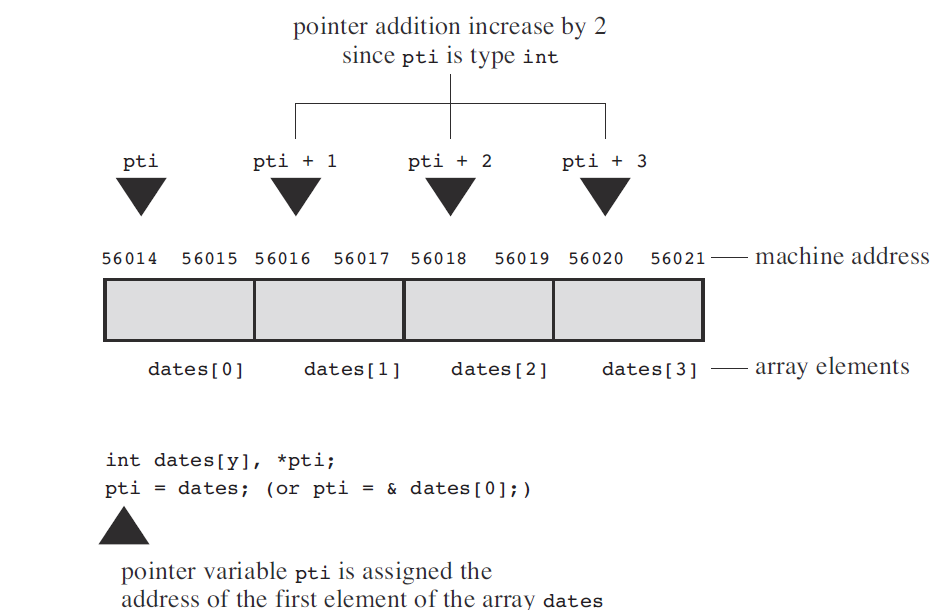
\includegraphics[width=0.85\textwidth]{Imagens/Imag02.png}
		%\caption*{Linguagem Python.}
	\end{figure}


\end{frame}


%=============================================================

\begin{frame}[fragile]
  \frametitle{Elementos de um vetor}
  \begin{block}{Exemplo 4}
  \begin{lstlisting}
  #include <stdio.h>
  int main() {
    int arr[] = {1, 2, 3, 4, 5};
    int *ptr = arr;
    printf("Endereco do array: %p\n",array);
    printf("Endereco do ponteiro: %p\n",&ptr);
    
    printf("Elemento %d\n", &arr[0]);
    printf("Elemento %d\n", &arr[1]);
    printf("Elemento %d\n", &arr[2]);
    printf("Elemento %d\n", &arr[3]);
    printf("Elemento %d\n", &arr[4]);
    
    
    printf("Elemento %d\n", *(ptr + 0));
    printf("Elemento %d\n", *(ptr + 1));
    printf("Elemento %d\n", *(ptr + 2));
    printf("Elemento %d\n", *(ptr + 3));
    printf("Elemento %d\n", *(ptr + 4));
        
    return 0;
  }
  \end{lstlisting}
  \end{block}
\end{frame}


%=============================================================

\begin{frame}[fragile]
  \frametitle{Soma dos elementos de um vetor}
  \begin{block}{Exemplo 5}
  \begin{lstlisting}
  #include <stdio.h>
  int main() {
    int arr[] = {1, 2, 3, 4, 5};
    int *ptr = arr;
    for (int i = 0; i < 5; i++) {
      printf("Elemento %d: %d\n", i, *(ptr + i));
    }
    return 0;
  }
  \end{lstlisting}
  \end{block}
\end{frame}


\section{Passagem por valor e por referência}

%============================================================


\begin{frame}[fragile]{}
  \frametitle{Usando funções por valor e por referência}
  \begin{block}{Exemplo 6: passando por valor}
  \begin{lstlisting}
  #include <stdio.h>
  int somar_valor(int,int);
  int main() {
    int a=5,b=4,c=0;

    c=somar_valor(a,b);
    printf("Resultado valor: %d\n",c);

    return 0;
  }
int somar_valor(int x,int y)
{
    int z=x+y;
    return z;

}  
  \end{lstlisting}
  \end{block}
\end{frame}

%============================================================

\begin{frame}[fragile]{}
  \frametitle{Usando funções por valor e por referência}
  \begin{block}{Exemplo 7: passando por referência}
  \begin{lstlisting}
  #include <stdio.h>
  void somar_ref(int*,int*);
  int main() {
  	int a=5,b=4;
    int *a_ptr=&a,*b_ptr=&b;
    somar_ref(a_ptr,b_ptr);
    printf("Resultado referencia: %d\n",*a_ptr);

    return 0;
  }
void somar_ref(int* x,int* y){
    *x=*x+*y;
}
  \end{lstlisting}
  \end{block}
\end{frame}

%============================================================


\begin{frame}{Referências}

\begin{itemize}
\item Prata, Stephen. C++ Primer Plus, 6th Edition. Índia: Pearson Education, 2012.
\item Prata, Stephen. C Primer Plus. Reino Unido: Pearson Education, 2013.
\end{itemize}





\end{frame}




\section{Ponteiros}
%==================================================================================
\begin{frame}
\frametitle{Ponteiros e vetores}

\begin{block}{Vetores}
\justifying
Vetores são sequências de elementos de um tipo de dado, armazenados em posições contíguas de memória, distribuídas em um número predeterminado de dimensões.
\end{block}

	\begin{figure}[h]
		\centering
		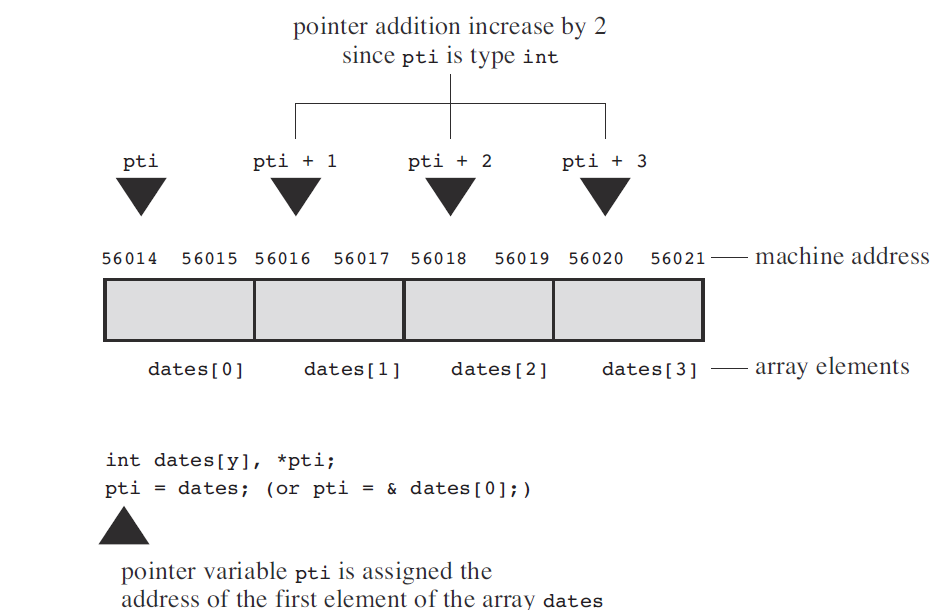
\includegraphics[width=0.75\textwidth]{Imagens/Imag02.png}
		%\caption*{Linguagem Python.}
	\end{figure}


\end{frame}

%==================================================================================


\begin{frame}[fragile]
  \frametitle{Referenciando os elementos dos vetores}
  
\begin{block}{Vetores}
\justifying
As referências aos elementos dos vetores são implementadas através da aritmética de ponteiros.
\end{block}

  \begin{block}{Exemplo: vetor 1-d}
  \begin{lstlisting}
#include <stdio.h>
#include <stdlib.h>

int main()
{
    int vet[5]={10,2,3,5,14};
    int *ptr_vet;

    ptr_vet=&vet;

    printf("%d\n",vet[1]);
    printf("%d\n",*(ptr_vet+1));

    return 0;
}
  \end{lstlisting}
  \end{block}
\end{frame}
%==================================================================================

\begin{frame}[fragile]
  \frametitle{Referenciando os elementos dos vetores}

  \begin{block}{Exemplo: vetor 2-d}
  \begin{lstlisting}
#include <stdio.h>
#include <stdlib.h>

int main()
{
    int vet[3][3]={{10,2,3},{5,14,-3},{9,6,4}};
    int *ptr_vet;

    int row=3,col=3,i,j;

    ptr_vet=&vet;
    i=1;
    j=2;

    printf("%d\n",vet[i][j]);

    printf("%d\n",*(ptr_vet + row*i + j));

    return 0;
}

  \end{lstlisting}
  \end{block}
\end{frame}

\section{Alocação}

%==================================================================================
\begin{frame}
\frametitle{Alocação de memória}


Existem três tipos de alocação:

\begin{itemize}
\justifying
\item \textbf{Estático:} a variável é alocada uma única vez, antes do início da execução do programa, e permanece alocada durante toda a execução.
\item \textbf{Automático:} a variável é alocada sempre que a execução da programação inicia o bloco no qual ela é declarada, permanecendo alocada até que o bloco seja finalizado. O valor inicial é indeterminado mas sempre que a declaração da variável é executada, ela assume o valor da sua expressão de iniciação, se houver, ou um valor indeterminado, em caso contrário.
\item \textbf{Por comando:} a alocação ocorre em decorrência da execução de comandos próprios de alocação de memória.
\end{itemize}



\end{frame}





%==================================================================================
\begin{frame}
\frametitle{Alocação de memória}


As funções de gerenciamento de memória permitem alocar, realocar e liberar espaços
de memória, e são declaradas no cabeçalho \textbf{stdlib.h}.

\begin{itemize}

\item void *malloc($size\_t \ tam$):\linebreak
Aloca espaço de memória de tamanho igual a \textbf{tam bytes}. O conteúdo do espaço alocado é indeterminado.



\item void *realloc(void *ptr,$size\_t \ tam$):\linebreak
Desloca o espaço apontado por \textbf{ptr}, realocando seu conteúdo em um novo espaço de tamanho igual a \textbf{tam bytes}.


\item void *calloc(unisgned int num, $size\_t \ tam$):\linebreak
Aloca uma quantidade de memória igual a \textbf{tam bytes}.


\end{itemize}


\begin{block}{free()}
Comando necessário para liberar memória.
\end{block}



\end{frame}


%==================================================================================
\begin{frame}
\frametitle{Vazamento de memória (Memory leak)}




\begin{block}{Memory leak}
O vazamento de memória é caracterizado pela existência de espaço de memória alocado,
mas que não pode ser acessado. Quando um espaço de memória é alocado pelas
funções \textbf{malloc}, \textbf{calloc} e \textbf{realloc}, ele permanece alocado até o término do programa
ou até que seja explicitamente desalocado. 
\end{block}


\end{frame}
%==================================================================================
\subsection{Malloc}


\begin{frame}[fragile]
  \frametitle{Exemplos de alocação de memória}
  

  \begin{block}{Exemplo: malloc}
  \begin{lstlisting}
#include <stdio.h>
#include <stdlib.h>

int main()
{
    int *mat;
    int lin=3,col=3,i,j;

    mat=(int *)malloc(lin*col*sizeof(int));

    *(mat + col*0 + 0)=2;

    for(i=0;i<lin;i++){
        for(j=0;j<col;j++){
            printf("%d\n",*(mat + col*i + j));
        }
    }
    return EXIT_SUCCESS;
}

  \end{lstlisting}
  \end{block}
\end{frame}

%==================================================================================
\subsection{Calloc}


\begin{frame}[fragile]
  \frametitle{Exemplos de alocação de memória}
  

  \begin{block}{Exemplo: calloc}
  \begin{lstlisting}
#include <stdio.h>
#include <stdlib.h>

int main()
{
    int *mat;
    int lin=3,col=3,i,j;

    mat=(int *)calloc(lin*col,sizeof(int));

    *(mat + col*0 + 0)=2;

    for(i=0;i<lin;i++){
        for(j=0;j<col;j++){
            printf("%d\n",*(mat + col*i + j));
        }
    }
    return EXIT_SUCCESS;
}


  \end{lstlisting}
  \end{block}
\end{frame}
%==================================================================================
\subsection{Realloc}

\begin{frame}[fragile]
  \frametitle{Exemplos de alocação de memória}
  

  \begin{block}{Exemplo: realloc}
  \begin{lstlisting}
#include <stdio.h>
#include <stdlib.h>

int main()
{
    int *mat,*vet;
    int lin=3,col=3,i,j;

    mat=(int *)calloc(lin*col,sizeof(int));

    *(mat + col*0 + 0)=2;

    vet=(int *)realloc(lin*col,sizeof(int));
    vet=mat;

    for(i=0;i<lin;i++){
        for(j=0;j<col;j++){
            printf("%d\n",*(vet + col*i + j));
        }
    }
    return EXIT_SUCCESS;
}

  \end{lstlisting}
  \end{block}
\end{frame}

%==================================================================================
\subsection{Memory leak}

\begin{frame}[fragile]
  \frametitle{Vazamento de memória}
  

  \begin{block}{Exemplo: memory leak}
  \begin{lstlisting}
#include <stdio.h>
#include <stdlib.h>

int main()
{
    int *mat,*vet;
    int lin=512,col=512,i,j;
    int tecla=1;



    while(tecla!=0){
        mat=(int *)calloc(lin*col,sizeof(int));

        printf("Digite: %d\n",tecla);
        scanf("%d",&tecla);
        //free(mat);

    }

    return EXIT_SUCCESS;
}


  \end{lstlisting}
  \end{block}
\end{frame}

%\input{contents/Estruturas}



%
%\input{contents/Contenido05}
%
%\input{contents/Contenido04}
%
%\input{contents/Contenido06}
%
%\input{contents/Contenido07}



\end{document}